\documentclass{article} % For LaTeX2e
\usepackage{nips13submit_e,times}
\usepackage{hyperref}
\usepackage{url}
\usepackage{amsmath}
\usepackage{graphicx}
%\documentstyle[nips13submit_09,times,art10]{article} % For LaTeX 2.09


\title{Large-Scale L1-Regularized and L2-Regularized Logistic Regression via a Stale Synchronous Parallel Parameter Server}


\author{
Yetian Xia\\
Computer Science Department\\
Carnegie Mellon University\\
Pittsburgh, PA 15213 \\
\texttt{yetianx@andrew.cmu.edu} \\
\And
Huanchen Zhang\\
Computer Science Department\\
Carnegie Mellon University\\
Pittsburgh, PA 15213\\
\texttt{huanche1@andrew.cmu.edu} \\
}

% The \author macro works with any number of authors. There are two commands
% used to separate the names and addresses of multiple authors: \And and \AND.
%
% Using \And between authors leaves it to \LaTeX{} to determine where to break
% the lines. Using \AND forces a linebreak at that point. So, if \LaTeX{}
% puts 3 of 4 authors names on the first line, and the last on the second
% line, try using \AND instead of \And before the third author name.

\newcommand{\fix}{\marginpar{FIX}}
\newcommand{\new}{\marginpar{NEW}}

\nipsfinalcopy % Uncomment for camera-ready version

\begin{document}


\maketitle

\begin{abstract}

\end{abstract}

\section{Introduction}

L1-regularized and L2-regularized logistic regression (LR) are widely used machine learning models that underlie many important applications in industry. A particular one that successfully applies these models is online advertising, including search advertising, contextual advertising, display advertising, and real-time bidding auctions [4]. According to eMarketer [10], the worldwide internet ad spending breaks the 100-billion mark in 2012 and is predicted to continue increasing by more than 20\% per year. Moreover, internet advertising is still the dominating revenue source for most search engines [7]. Most notably, Google earned \$36.4 billion from advertising alone, accounting for 96\% of its total revenue in 2011 [11].

The most common financial model, adopted by Google, Yahoo, and Microsoft [7], for online advertising is called “cost-per-click” billing. Essentially, the model states that advertisers (sponsors) pay the search engine company whenever a user clicks their ads [7]. As a result, the ability to efficiently and adaptively learn models that can quickly and accurately predict ad click-through rates has been playing a key role of revenue boost for those companies [4].

Three practical issues need to be resolved for ad click prediction systems to achieve good performance: sparsity, scalability and adptiveness. First, in such applications, the number of features is usually very large, resulting in high-dimensional data (examples). However, since the number of training examples is limited, logistic regression tends to overfit. A common way to reduce overfitting is through regularization, namely L1-norm and L2-norm regularization. The L2-norm regularization has the advantage of being able to reduce to a convex optimization problem that is always differentiable, while the L1-norm regularization is more attractive for dealing with high-dimensional data because it implicitly embeds feature selection in the classification process [3].

The second practical issue is scalability. Scalability is important to industrial applications because of both massive data volume and massive model size [1]. A typical industrial application nowadays is required to learn and predict billions of instances with high-dimensional feature space per day [4]. Meanwhile, observations show that increasing the scale of machine learning models can significantly improve classification accuracy [5]. The most natural way to address scalability is through parallelism. A number of distributed systems specifically optimized for machine learning have emerged recently [1] [2] [5], along with some theoretical work on consistency models for distributed ML [1] [9]. We will discuss some of these systems in sections 2. For this project, we use Petuum [2], an open source large-scale ML framework currently being developed at CMU, as the centralized shared parameter server to apply iterative-convergent methods (specifically, distributed gradient computation) to realize regularized LR models in large scale.

The final practical issue to be considered is adaptiveness, which means that the existing model is periodically refined through learning of the data obtained from the recent prediction results. Adaptiveness typically requires online algorithms where data is provided by a streaming service. In other words, each training example only needs to be considered once.

Despite that large-scale regularized logistic regression is widely adopted in proprietary systems, there is a lack of open source implementation. This project aims to fill in this need by implementing large-scale L2-regularized LR using stochastic gradient ascent (descent) and L1-regularized LR using subgradient method on a distributed ML framework, namely Petuum [2]. Our contribution also includes providing first-hand experience with Petuum, which might be valuable for Petuum to evolve to a mature ML-specific distributed system. Section 2 provides background and related work of LR algorithms and parallel (distributed) ML frameworks; Section 3 describes our algorithms and implementation details; Section 4 evaluates the performance of our system; Section 5 concludes. 

\section{Related Work}
\label{gen_inst}

In response to the unprecedented scalability challenges, various distributed ML frameworks, such as Google Brain [5], GraphLab [8], and SSPtable [1], have emerged recently. One popular idea is to relax synchronization requirements to overcome the inherent sequential nature of some ML models (e.g. stochastic gradient descent) to increase throughput. For example, Google implemented the "downpour SGD" algorithm on their distributed ML framework "Google Brain", which not only parallelizes computation across multiple model instances, but also within each one [5]. Specifically, training data is divided into a number of partitions and each partition only feeds to a single model instance. Meanwhile, all the model replicas share a centralized parameter sever that is also sharded. In other words, a single machine (or thread) within a particular model instance is only responsible for updating one shard of the parameter server using a single partition of training data [5]. In our project, we leverage such design for parallelization. In addition, we also include proper consistency guarantees, namely bounded staleness, to further gain throughput improvements.

Of the all the consistency models, ranging from no consistency to sequential consistency, bounded staleness consistency model, a variant of eventual consistency, has recently proved to work the best for iterative-convergent algorithms (e.g. SGD) especially with sparse data [1] [2] [9] [12]. A notable example is the Stale Synchronous Parallel (SSP) model presented by [1], as opposed to the traditional Bulk Synchronous Parallel (BSP) model. In SSP, a model replica is allowed to lead or lag other replicas by at most s iterations, where s is a preconfigured number, while the convergence of the algorithm is still guaranteed [1]. In this way, communication between a local replica and the parameter server is only required when the staleness of the local replica is more than s iterations [9]. Therefore, the network communication cost is significantly reduced, resulting in higher throughput [5].

Petuum [5], the distributed ML framework used in this project, is a general-purpose platform designed for big learning. In particular, it is optimized to solve loss function minimization problems that have an embedded iterative-convergent nature [5]. Similar to its precedence, Petuum provides a distributed key-value store as the shared parameter server among threads. In addition, Petuum also introduces a variable scheduler to dynamically maintain load balancing among worker machines. Moreover, Petuum offers a number of bounded-staleness consistency models, including SSP and value-bounded consistency, to reduce network cost while remaining error-resistant. Other system-level optimizations associated with Petuum include process-level and thread-level caching and out-of-core storage support [5].

Algorithmwisely, despite that L1-regularized LR is more difficult than L2-regularized LR because of its indifferentiability, researchers have developed a number of efficient methods to solve the problem. Note that although gradient does not exist with L1-regularization, subgradient exists and can be used instead of gradient in the SGD algorithm [15]. Shalev-Shwartz and Tewari [16] transformed the indifferentiable objective function into an equivalent problem with a twice-differentiable regularizer. Then a great number of methods, such as gradient descent, coordinate descent and second-order methods, can be applied to solve this new optimization problem. According to Schmidt et al.[15], such approach can be considered as unconstrained approximations. Schmidt et al.[15] also mentioned another approach which first reduces the problem to a constrained optimization problem and then sovles it.

\section{Methods}
\label{headings}

In this section, we first present a derivation of the algorithms chosen to implement large-scale L2-regularized and L1-regularized LR respectively. We then describes our system design and implementation based on Petuum [2] in detail.

\subsection{Stochastic Gradient Ascent (Descent) for Logistic Regression}

The following derivation refers to [6]. Suppose that the training set has n examples $\vec{x_1}$ to $\vec{x_n}$, each having a dimension of d. Let $y_1$ to $y_n$ denote the corresponding binary labels, i.e. $y_i \in \{0, 1\}$ for $\forall i = 1, ..., n$. The logistic function is defined as $\sigma(z) = \frac{1}{1+e^{-z}}$. The parameters associated with the LR model are $w_0$ and $\vec{w} = (w_1, ..., w_d)$. Let ($\vec{x}$, $y$) be a test sample, then we have the following probability model for logistic regression:

\begin{align*}
    p = P(y=1 | \vec{x}; w_0, \vec{w}) &= \sigma(w_0 + \sum\limits_{j=1}^d w_jx_j) = \frac{1}{1 + e^{-(w_0 + \vec{w}^\top\vec{x})}}\\
    P(y=0 | \vec{x}; w_0, \vec{w}) &= 1 - p = \frac{e^{-(w_0 + \vec{w}^\top\vec{x})}}{1 + e^{-(w_0 + \vec{w}^\top\vec{x})}}
\end{align*}


Using the above probablity model, we can compute the log odds as the following:

\begin{equation}
  ln\frac{p}{1-p} = w_0 + \vec{w}^\top\vec{x}
\end{equation}

and thus we have the classification rule for LR:
\begin{align*}
  y &= 1, \ \ \ \ \ if \ w_0 + \vec{w}^\top\vec{x} \geq 0\\
  y &= 0, \ \ \ \ \ otherwise.
\end{align*}

Let $\vec{w^*} = (w_0, \vec{w})$ and $\vec{x^*} = (1, \vec{x})$. Now the classification criteria becomes whether $\vec{w^*}^\top\vec{x^*} \geq 0$ or not. For notation simplicity, we denete $\vec{w^*}$ and $\vec{x^*}$ by $\vec{w}$ and $\vec{x}$ respectively from now on.

Given the training set, we learn the LR parameters using MLE (Maximum Likelyhood Estimator) method. Specifically, we want to maximize the following log joint conditional likelihood:

\begin{equation}
  LJCL = ln\prod\limits_{i=1}^nP(y_i | \vec{x_i}; \vec{w}) = \sum\limits_{i=1}^nlnP(y_i | \vec{x_i}; \vec{w})
\end{equation}

For each parameter $w_j$, the partial derivative of LJCL with respect to $w_j$ is:

\begin{equation}
\begin{split}
  \frac{\partial}{\partial w_j} LJCL &= \sum\limits_{i=1}^n\frac{\partial}{\partial w_j}lnP(y_i | \vec{x_i}; \vec{w})\\
  &= \sum\limits_{i:y_i=1}\frac{\partial}{\partial w_j}lnp_i + \sum\limits_{i:y_i=0}\frac{\partial}{\partial w_j}ln(1-p_i) = \sum\limits_{i:y_i=1}\frac{1}{p_i}\frac{\partial}{\partial w_j}p_i + \sum\limits_{i:y_i=0}\frac{1}{1-p_i}(-\frac{\partial}{\partial w_j}(1-p_i))\\
  &= \sum\limits_{i:y_i=1}(1+e^{-\vec{w}^\top\vec{x_i}})\frac{-1}{(1+e^{-\vec{w}^\top\vec{x_i}})^2}\frac{\partial}{\partial w_j}e^{-\vec{w}^\top\vec{x_i}} + \sum\limits_{i:y_i=0}\frac{(1+e^{-\vec{w}^\top\vec{x_i}})}{e^{-\vec{w}^\top\vec{x_i}}}\frac{1}{(1+e^{-\vec{w}^\top\vec{x_i}})^2}\frac{\partial}{\partial w_j}e^{-\vec{w}^\top\vec{x_i}}\\
  &= \sum\limits_{i:y_i=1}\frac{e^{-\vec{w}^\top\vec{x_i}}}{1+e^{-\vec{w}^\top\vec{x_i}}}x_{ij} + \sum\limits_{i:y_i=0}\frac{-1}{1+e^{-\vec{w}^\top\vec{x_i}}}x_{ij} = \sum\limits_{i:y_i=1}(1-p_i)x_{ij} + \sum\limits_{i:y_i=0}(-p_i)x_{ij}\\
  &= \sum\limits_{i=1}^n(y_i-p_i)x_{ij}
\end{split}
\end{equation}

Instead of evaluating $\sum\limits_{i=1}^n(y_i-p_i)x_{ij}$ for all $j$, which has a complexity of
$O(nd)$, we compute a random approximation of the partial derivatives (gradient):
\begin{equation}
  \frac{\partial}{\partial w_j} LJCL = \sum\limits_{i=1}^n(y_i-p_i)x_{ij} \approx n(y_i-p_i)x_{ij}
\end{equation}
where $i$ is selected randomly from the training set. Therefore, the update rule for parameter $w_j$ using stochasitc gradient ascent is:
\begin{equation}
  w_j = w_j + \lambda (y_i-p_i)x_{ij}
\end{equation}
where $n$ is embedded in $\lambda$ since it is a constant.

Stochastic gradient ascent (descent) is particularly useful for sparse data (where most of the $x_j$'s are 0) because only a few parameters need to be updated for each iteration [6]. One practical issue to be noticed is that since the learning rate $\lambda$ is kept constant for every parameter, it is necessary to normalize the magnitude of every feature beforehand [6].

\subsubsection{L2-Regularization}

As mentioned in section 1, we apply regularization to prevent overfitting, i.e. we penalize on the magnitude of the parameters. For L2-regularization, instead of maximizing $LJCL$, we now maximize $LJCL - \mu ||\vec{w}||_2^2$ to obtain MLE, where $\mu$ quantifies the penalty scale. Accordingly, the update rule for parameter $w_j$ becomes:
\begin{equation}
  w_j = w_j + \lambda [(y_i-p_i)x_{ij} - 2\mu w_j]
\end{equation}


\subsubsection{L1-Regularization}
For L1-regularization, we now maximize $LJCL - \mu ||\vec{w}||_1$ to obtain MLE.
We use the subgradient decient method to solve this problem because of its simplicity and efficiency. A vector $\textup{g} \in \textbf{R}^n$ is a subgradient of $\textup{f}:\textbf{R}^n \rightarrow \textbf{R}$ at $x_0 \in \textbf{R}^n$ if for all $z \in \textbf{R}^n$,
\begin{equation}
f(z) \ge f(x_0) + g^T(z-x_0)
\end{equation}
And [15] gives the formula for calculating the subgradient for $l1$-regularized logistic regression.
\begin{equation}
\bigtriangledown f(\omega_i) = \left\{\begin{matrix}
\bigtriangledown LJCL(\omega_i) + \mu sign(\omega_i) & |\omega_i| > 0\\ 
\bigtriangledown LJCL(\omega_i) + \mu & \omega_i=0,\bigtriangledown LJCL(\omega_i)<-\mu\\ 
\bigtriangledown LJCL(\omega_i) - \mu & \omega_i=0,\bigtriangledown LJCL(\omega_i)>\mu\\ 
0 & \omega_i=0, -\mu \le \bigtriangledown LJCL(\omega_i) \le \mu
\end{matrix}\right.
\end{equation}

We can replace the gradient in the previous section with the above subgradient to get the updating rule for L1-regularized LR.

\subsection{Parallelization on Petuum}
Although stochastic gradient descent is efficient, the methods are inherently sequential, which makes it impractical to apply on huge amount of data. In order to extend SGD to large data sets, we parallelize the computation using the Petuum framework. We partition both training data and parameters in a similar way Google Brain [5] does to achieve higher throughput and less training time.

First, we need to configure Petuum. Fortunately, Petuum (the latest version) maintains a centralized parameter server, which is shared among workers asynchronously, along with a spectrum of consistency models. We decided to adopt the most recent SSP consistency model for this project. The key idea of the design is to orthogonally parallelize training data and gloabla parameters at the same time. Specifically, we divide the training data into a number of subsets and assign each subset to a bunch of workers, each of which is responsible for updating a disjoint set of parameters. Essentially, workers communicate with each other through the parameter server and will keep updating the parameters until they converge.

\begin{figure}[h]
\begin{center}
%\framebox[4.0in]{$\;$}
%701.png
\fbox{\rule[-.5cm]{0cm}{4cm} 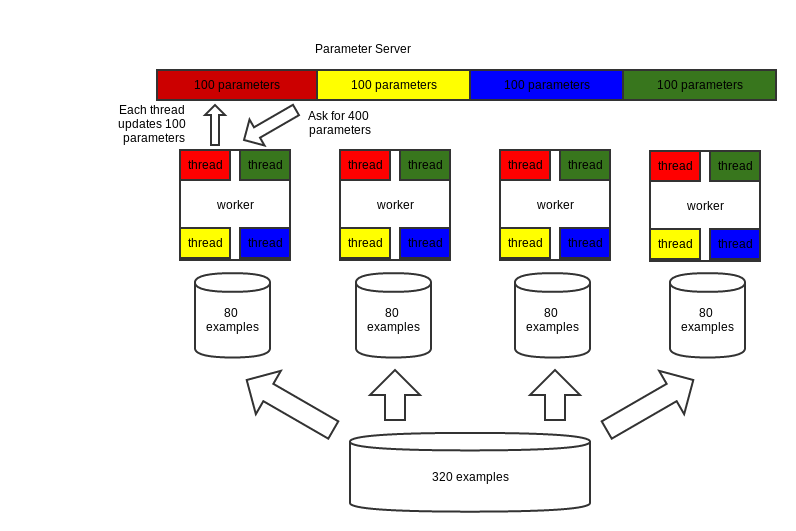
\includegraphics[width=280px]{701.png} \rule[-.5cm]{4cm}{0cm}}
\end{center}
\caption{A normal working example.}
\label{example}
\end{figure}
For example, suppose we want to estimate 400 parameters on 320 training examples. As shown in Figure \ref{example}, we have a parameter server shared by four workers, while each worker also contains 4 worker threads. Then each worker thread is only responsible for updating 100 parameters using its assigned 80 training examples. In a typical round, if a work discovers that some of its worker threads are $s$ iterations behind (or beyond), the worker is required to synchronize with the parameter server, and force all the worker threads to update accordingly. Convergence is guaranteed by this SSP model, as proved in [1] [2] [9].

Our method can be regarded as a variant of Shotgun[13], a parallelized method of Shooting[14] algorithom. The main differences are: 1) we update global parameters asychronously; 2) each worker thread updates parameters using only a subset of the training data; 3) each worker thread is responsible for a subset of the parameters. 

\section{Experiments}
\label{others}
We will use UCI Pima Indians Diabetes datasets [17] in the LIBSVM [18] format for testing and debugging purpose.
We will also use a Wikipedia dataset that has 3 million instances, as suggested by the TA (Dani). For evaluation, we will first run the logistic regression using a single thread on a single machine, so that it gives us the baseline of converge time for a certain accuracy because there is no consistency issue (i.e. update conflicts) related. We will then run the LR using multi-threads (one thread per core) to simulate the distributed environment. We will plot the converge time against the number of threads (cores), and we anticipate to see a close-to-linear speed up as the number of threads goes up.

If time and resource permit, we will set up our system on a public cluster (e.g. Amazon EC2) and test on the huge original dataset to obtain a more real and accurate performance measure.

\section{Conclusion}


\subsubsection*{References}

\small{
[1] Ho, Q., Cipar, J., Cui, H., Kim, J. K., Lee, S., Gibbons, P. B., Gibson, G. A., Ganger, G. R., \& Xing, E. P. (2013). More Effective Distributed ML via a Stale Synchronous Parallel Parameter Server. In {\it Advances in Neural Information Processing Systems} (pp. 1223-1231).

[2] Dai, W. et al. (2013). Petuum: A Framework for Iterative-Convergent Distributed ML. {\it arXiv preprint arXiv:1312}.7651.

[3] Liu, J., Chen, J., \& Ye, J. (2009). Large-scale sparse logistic regression. In {\it Proceedings of the 15th ACM SIGKDD international conference on Knowledge discovery and data mining} (pp. 547-556). ACM.

[4] McMahan, H. B. et al. (2013). Ad click prediction: a view from the trenches. In {\it Proceedings of the 19th ACM SIGKDD international conference on Knowledge discovery and data mining} (pp. 1222-1230). ACM.

[5] Dean, J. et al. (2012). Large Scale Distributed Deep Networks. In {\it NIPS} (pp. 1232-1240).

[6] Elkan, C. Maxinum Likelihood, Logistic Regression, and Stochastic Gradient Training. http://cseweb.ucsd.edu/~elkan/250B/logreg.pdf

[7] Richardson, M., Dominowska, E., \& Ragno, R. (2007). Predicting clicks: estimating the click-through rate for new ads. In {\it Proceedings of the 16th international conference on World Wide Web} (pp. 521-530). ACM.

[8] Low, Y., Bickson, D., Gonzalez, J., Guestrin, C,. Kyrola, A., \& Hellerstein, J. M. (2012). Distributed GraphLab: a framework for machine learning and data mining in the cloud. {\it Proceedings of the VLDB Endowment}, 5(8), 716-727.

[9] Wei, J., Dai, W., Kumar, A., Zheng, X., Ho, Q., \& Xing, E. P. (2013). Consistency Models for Distributed ML with Theoretical Guarantees. {\it arXiv preprint arXiv:1312}.7869.

[10] Growth in digital to remain in double digits through 2015. http://www.emarketer.com/Article/Digital-Account-One-Five-Ad-Dollars/1009592

[11] Miranda M. How Google Made \$37.9 Billion in 2011 http://searchenginewatch.com/article/2140712/How-Google-Made-37.9-Billion-in-2011

[12] Niu, F., Recht, B., Ré, C., \& Wright, S. J. (2011). Hogwild!: A lock-free approach to parallelizing stochastic gradient descent. {\it Advances in Neural Information Processing Systems, 24}, 693-701.

[13] Bradley, J. K., Kyrola, A., Bickson, D., \& Guestrin, C. (2011). Parallel coordinate descent for l1-regularized loss minimization. arXiv preprint arXiv:1105.5379.

[14] Fu, W. J. (1998). Penalized regressions: the bridge versus the lasso. Journal of computational and graphical statistics, 7(3), 397-416.

[15] Schmidt, M., Fung, G., \& Rosales, R. (2007). Fast optimization methods for l1 regularization: A comparative study and two new approaches. In Machine Learning: ECML 2007 (pp. 286-297). Springer Berlin Heidelberg.

[16] Shalev-Shwartz S., Tewari A.. 2011. Stochastic Methods for l1-regularized Loss Minimization. J. Mach. Learn. Res. 12 (July 2011), 1865-1892.

[17] Bache, K. \& Lichman, M. (2013). UCI Machine Learning Repository [http://archive.ics.uci.edu/ml]. Irvine, CA: University of California, School of Information and Computer Science.

[18] Chih-Chung Chang and Chih-Jen Lin, LIBSVM : a library for support vector machines. ACM Transactions on Intelligent Systems and Technology, 2:27:1--27:27, 2011. Software available at http://www.csie.ntu.edu.tw/~cjlin/libsvm. 
}

\end{document}
